\documentclass[11pt]{article}

\usepackage{natbib}
\usepackage{graphicx}
\usepackage{mathpartir}

\newcommand{\inbnd}{\mathord -}
\newcommand{\outbnd}{\mathord +}
\newcommand{\cnf}[1]{\ensuremath{\operatorname{\maths{#1}}}}
\newcommand{\cnc}[1]{\ensuremath{\mathsf{#1}}}
\newcommand{\mcl}[1]{\ensuremath{\mathcal{#1}}}
\newcommand{\nxt}[4]{\xymatrix@C=3.5em{{#1}\ar@{=>}[r]^{#2\##3}&{#4}}}
\newcommand{\seq}{\mathbin{;}}
\newcommand{\encrypt}[2]{\ensuremath{\{#1\}_{#2}}}
\newcommand{\sep}{\colon}
\newcommand{\seqa}{\mathbin{;\!;}}
\newcommand{\join}[3]{#1\hookrightarrow#3\hookleftarrow#2}
\newcommand{\sig}[2]{\ensuremath{[\![#1]\!]_{#2}}}
\newcommand{\act}[1]{\stackrel{#1}{\Rightarrow}}
\newcommand{\all}[1]{\mathop{\forall#1\mathpunct.}}
\newcommand{\some}[1]{\mathop{\exists#1\mathpunct.}}
\newcommand{\skp}{\cnc{SKIP}}
\newcommand{\env}{\cnc{SIG}}
\newcommand{\usm}[2]{\cnc{USM}\;#1\;#2}
\newcommand{\UV}[2]{\cnc{usm}_{#1}\;#2}
\newcommand{\UU}[2]{\cnc{U}_{#1}\;#2}
\newcommand{\lkim}[3]{\cnc{KIM}_{#1}\;#2\;#3}
\newcommand{\LV}[3]{\cnc{kim}^{#1}_{#2}\;#3}
\newcommand{\LL}[3]{\cnc{K}^{#1}_{#2}\;#3}
\newcommand{\NV}[1]{\cnc{n}_{#1}}
\newcommand{\NN}[1]{\cnc{N}_{#1}}
\newcommand{\at}[2]{\mathop{@_{#1}}{#2}}
\newcommand{\eval}[3]{\mcl{E}(#1,#2,#3)}
\newcommand{\step}[1]{\stackrel{#1}{\longrightarrow}}

\newcommand{\squash}{\parskip=0pt\itemsep=0pt}

\title{stairCASE Measurement Architecture}
\author{Perry Alexander}

\begin{document}

\maketitle

\section{Architecture}

\subsection{Ground Station}

\begin{itemize}
  \squash
\item seL4 instance running on ODROID
\item User Virtual Platform (UVP) on seL4 VMM
\item Linux instance on seL4 VM
\item User AM as Linux process
\item UxAS as Linux process
\item Platform AM as CAmkES component
\item Attestation Manager (seL4AM)
\end{itemize}

\begin{figure}[hbtp]
  \centering
  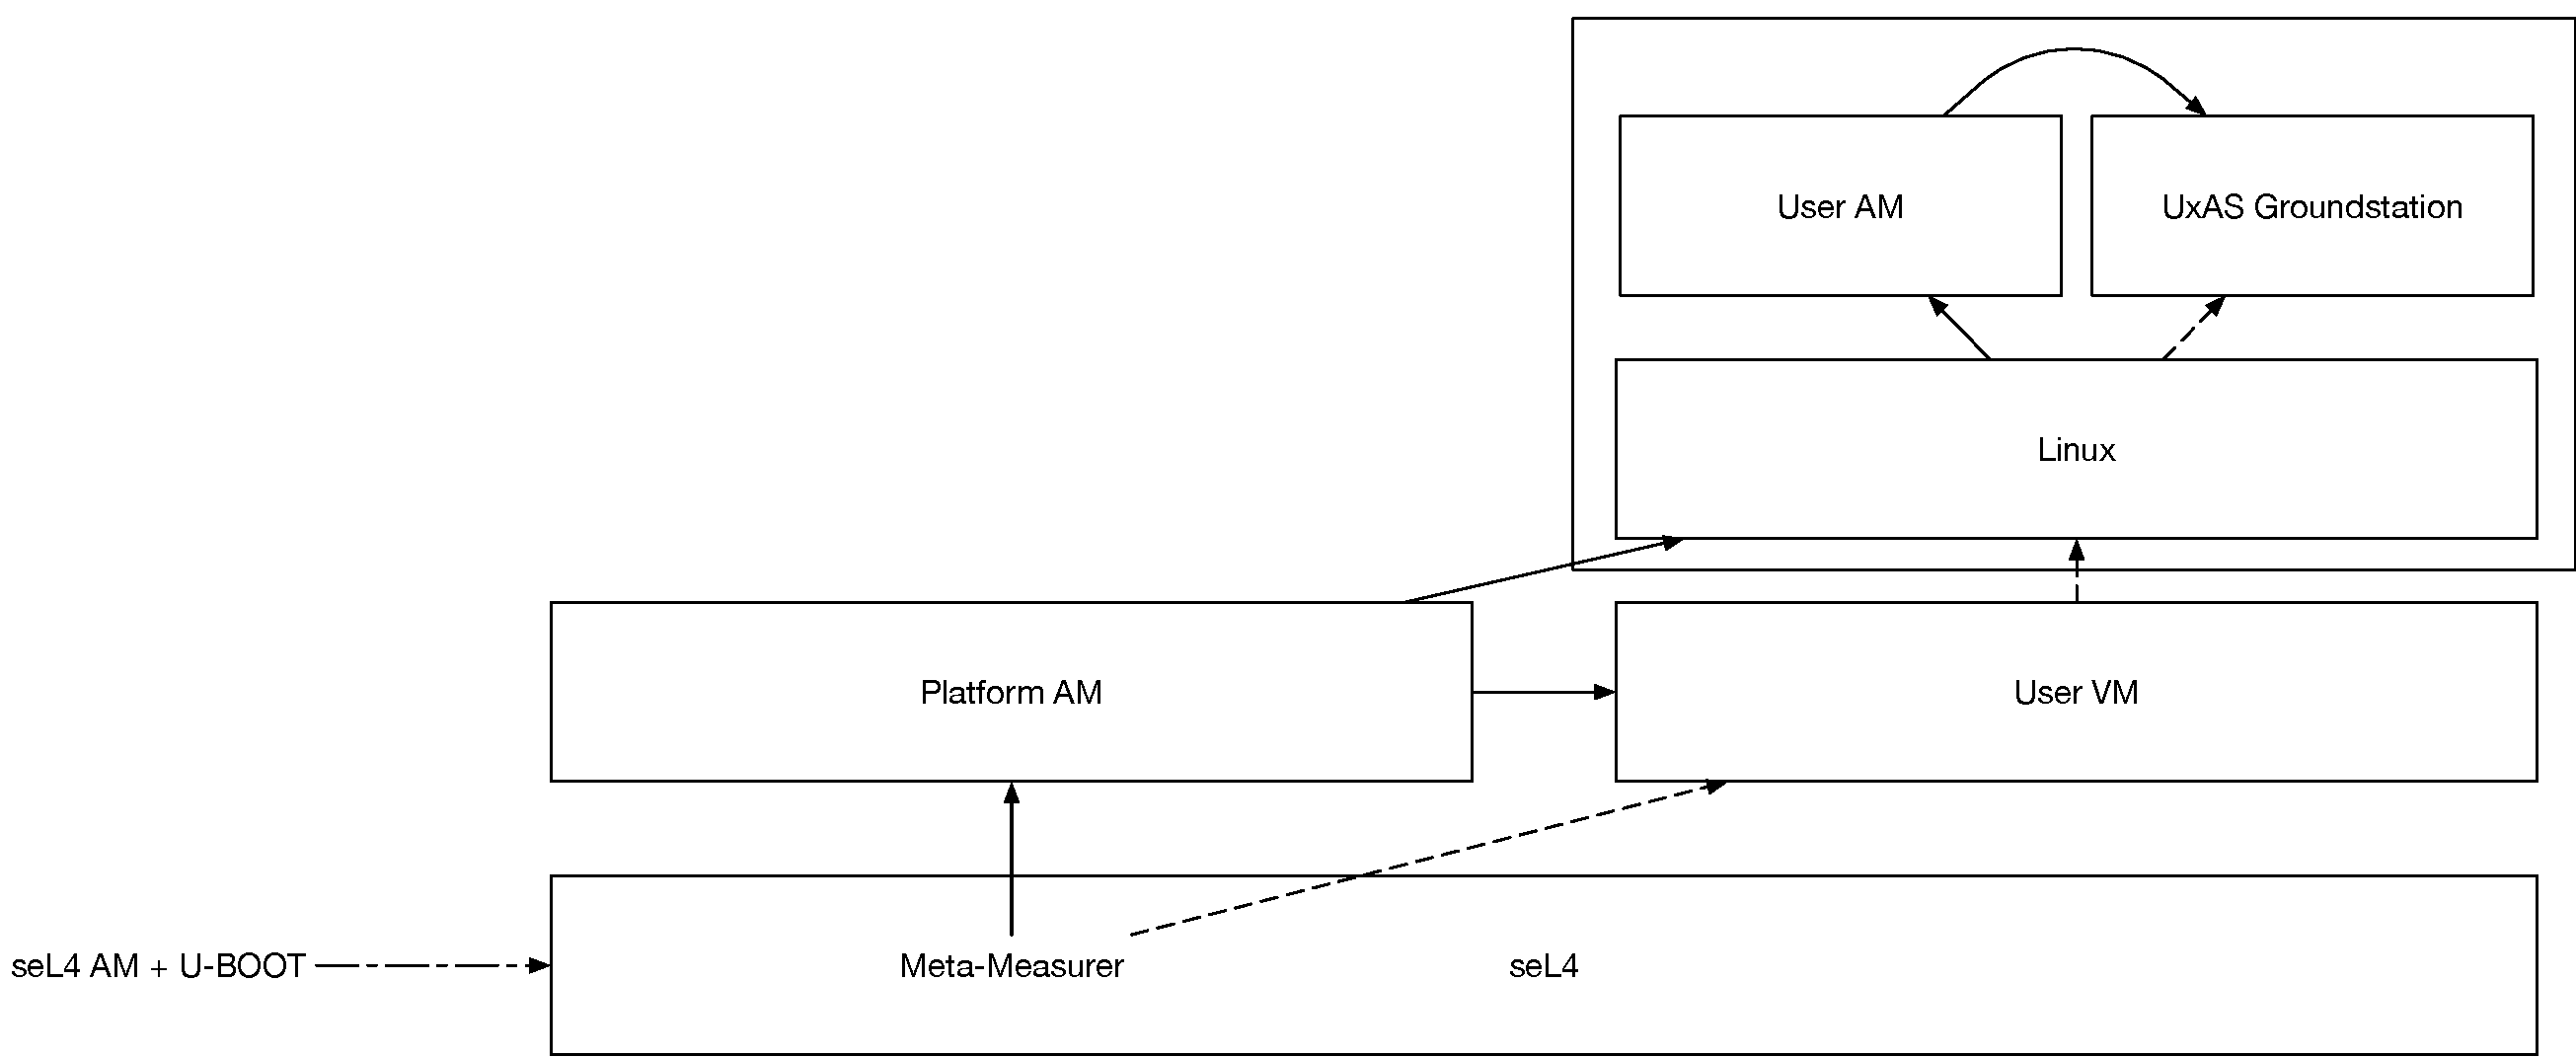
\includegraphics[width=\textwidth]{architecture.pdf}
  \caption{Measurement \& Attestatin Architecture}
  \label{fig:architecture}
\end{figure}

\subsection{Mission board}

\begin{itemize}
\item Mission AM as dictated by mission board designers
\end{itemize}

\subsection{Roots of Trust}

\begin{itemize}
  \parskip=0pt\itemsep=0pt
\item RoT for Measurement - UBOOT
\item RoT for Reporting - place key
\item RoT for Storage - ??
\end{itemize}

\section{Places}

\begin{itemize}
  \squash
\item Mission AM - Appraisal only.  Makes requests of ground station
  AMs and appraises results.  No mutual attestation at this time, but
  could add later if desirable.
\item seL4 AM - Hashes the seL4 instance at startup and performs
  runtime integrity measurement. This may conflate with what U-BOOT
  currently does.  Note that UBOOT performs a signature check and does
  not currently measure the seL4 imagage.  Potentially the root of
  trust for measurement.
\item Platform AM - Hashes the UVP VM at startup and performs runtime
  integrity measurement. Is hashed as a part of the seL4IM
  measurement.  Consider meta-measurer runnning as CAmkES component to
  ensure integrity.  seLAM might do this as well.
\item UVP AM - Hashes the UxAS instance at startup and performs
  runtime integrity measurement.  Is hashed as a part of the Platform
  measurement.  Serves as the interface to the attestation platform.
\end{itemize}

\section{Boot Measurement Story}

\begin{enumerate}
  \squash
\item UVP Linux VM hashes and starts UVP AM.
\item UVP Linux VM hashes and starts UxAS groundstation.  Makes UVP AM
  aware of UxAS. UVP AM measures UxAS. 
\end{enumerate}


\begin{enumerate}
  \squash
\item UBOOT starts seL4 AM and seL4.  seL4 AM measures seL4 image and
  stores in TrustZone. seL4 AM is made aware of seL4. seL4 AM may be a
  part of UBOOT.  UBOOT has a built-in SHA-256 capability.
\item seL4 starts and measures Platform AM as CAmkES component.
\item seL4 measures and starts User Virtual Platform (UVP) consisting
  of Linux VM and a RAMdisk.

  \begin{enumerate}
    \squash
  \item Hashes and starts the Linux kernel as VM
  \item Hashes and mounts RAMDisk
  \end{enumerate}
  
  sel4 Makes the Platform AM CAmkES component aware of UVP and
  RAMDisk.

\item UVP Linux VM hashes and starts UVP AM from a RAMDisk image.
\item UVP Linux VM hashes and starts UxAS groundstation from a RAMDisk
  image.  Makes UVP AM aware of UxAS executing.
\item UVP AM measures UxAS and begins accepting attestation requests
  from Mission AM
\end{enumerate}

\section{Runtime Measurement Story}

\begin{enumerate}
\item seL4 AM measures sel4 instance
\item seL4 AM measures Platform AM (speculative)
\item Platform AM measures UVP VM and UVP AM
\item UVP AM measures UxAS groundstation and serves as interface to
  mission platform AM 
\end{enumerate}

\section{Appraisal Story}

\begin{itemize}
  \squash
\item Mission board is aware of the UVP AM and sends requests to it.
\item UVP AM is aware of Platform AM and seL4IM and sends requests to
  them as required by Mission Board requests
\item Two kinds of attestation requests
  \begin{itemize}
  \item Shallow attestation requests invoke UVP AM to measure the
    application and local platform
  \item Deep attestation requests invoke UVP AM to make requests of
    Platform AM and seL4IM 
  \end{itemize}
\end{itemize}


\section{APDT terms}

\begin{mathpar}
  \mathsf{seL4Meas} = \at{\mathsf{seL4AM}}{(\NV{1}\seq\usm{\mathsf{seL4Hash}}{\epsilon}\seq\lkim{\mathsf{platformAM}}{\mathsf{pkim}}{\epsilon}\seq\env)}

  \mathsf{platformMeas} = \at{\mathsf{platformAM}}{(\NV{2}\seq\usm{\mathsf{seL4Meas}}{\NV{1}}\seq\lkim{\mathsf{userAM}}{\mathsf{ukim}}{\epsilon}\seq\env)}

\end{mathpar}

\section{Open Questions}
        
\begin{itemize}
  \squash
\item RoT for Storage - where can we put measurements and keys that
  provides confidentiality and integrity?
  \begin{itemize}
    \squash
  \item TrustZone proto-TPM - Need to jack with TrustZone.  Possibly
    store first measurement here and use CAmkES component for the
    rest.
  \item CAmkES component - Need to store measurements prior to seL4 start
  \end{itemize}
\item Hosting and running KIMs - what will our KIMs be and how will they function?
  \begin{itemize}
    \squash
  \item LKIM for UVP AM
  \end{itemize}
\end{itemize}

\section{Odds and Ends}

\begin{itemize}
  \squash
\item UBOOT can hash images
\item UBOOT runs through TrustZone in some way that we need to
  understand
\item seL4 VMM can start with 2 VMs
  \begin{itemize}
    \squash
  \item one is an OS Kernel
  \item one is typically a RAM Disk
  \end{itemize}
\item New boot structure
  \begin{itemize}
    \squash
  \item start the kernel
  \item mount the RAMDisk
  \item start the user apps from the ramdisk
  \end{itemize}
\end{itemize}

\end{document}
